\documentclass{article}
\usepackage[utf8]{inputenc}
\usepackage[legalpaper, portrait, margin=1in]{geometry}
\usepackage{enumitem}
\usepackage{graphicx}
\newcommand{\probP}{\text{I\kern-0.35em P}}


\title{CS 156a FINAL}
\author{Cason Shepard}

\begin{document}

\maketitle

\section*{problem 1}
We will use the formula $d = \frac{Q(Q+3)}{2}$. Since $Q = 10$, we get $d = \frac{130}{2} = 65$. This is not an option.\\\\
\textbf{The answer is [e]}

\section*{problem 2}
Consider the average of two logistic functions. Sometimes the results will simply not be logistic.\\\\
\textbf{The answer is [d]}

\section*{problem 3}
In this instance, d is false. This is because we cannot generalize to all instances. When over fitting occurs, we have a hypothesis that generates a very small $E_{in}$, but a large $E_{out}$. Consider we have a small training set, but a very large test set. In this case we can expect our hypothesis function to be very well fitted to the training data, thus $E_{in}$ will be very small. However, due to our small training set, the $E_{out}$ could be very large. In this case, we might be wary that our data is over fitted, but a small training set prevents this determination. Thus, we cannot \textit{always} determine if the data is over fitted through comparing $E_{in}$ and $E_{out}$.\\\\
\textbf{The answer is [d]}

\section*{problem 4}
Stochastic noise is random noise that is a part of the target function we are trying to evaluate, where as we view deterministic noise as a byproduct of the hypothesis we choose. Thus, stochastic noise is independent of the hypothesis set.\\\\
\textbf{The answer is [d]}

\section*{problem 5}
We know that $w_{reg}^Tw_{reg} = C$. So, from the textbook, we know that $w_{reg} = w_{lin}$ to satisfy the equation.\\\\
\textbf{The answer is [a]}

\section*{problem 6}
It is known that augmented error constraints can be used to measure the goodness of a soft-order constraint. Thus, soft-order constraints can be translated into augmented error.\\\\
\textbf{The answer is [b]}

\section*{problem 7}
After running the code attached, the lowest $E_{in}$ was found for the 8-versus-all classifier.
\begin{enumerate}[label=(\alph*)]
    \item $E_{in} = 0.076$
    \item $E_{in} = 0.091$
    \item $E_{in} = 0.088$
    \item $E_{in} = 0.074$
    \item $E_{in} = 0.088$
\end{enumerate}
\textbf{The answer is [d]}

\section*{problem 8} 
After running the code attached, the lowest $E_{out}$ was found for the 1-versus-all classifier.
\begin{enumerate}[label=(\alph*)]
    \item $E_{out} = 0.107$
    \item $E_{out} = 0.022$
    \item $E_{out} = 0.099$
    \item $E_{out} = 0.083$
    \item $E_{out} = 0.100$
\end{enumerate}
\textbf{The answer is [b]}

\section*{problem 9}
Using the 5-versus-all classifier, the following $E_{out}$ was produced:
\begin{enumerate}[label = ]
    \item Non-Transformed: $E_{out} = 0.079\textbf{72097658196313}$
    \item Transformed: $E_{out} = 0.079\textbf{22272047832586}$
\end{enumerate}
The transformed improved the 5-versus-all out-of-sample performance by $0.6\%$ Thus, e is true.\\\\
\textbf{The answer is [e]}

\section*{problem 10}
After running the code attached, the following values for $E_{in}$ and $E_{out}$ was produced:
\begin{enumerate}[label =]
    \item Lambda: 0.01
    \item $E_{out}: 0.0283$
    \item $E_{in}: 0.0045$
    \item Lambda: 1
    \item $E_{out}: 0.0259$
    \item $E_{in}: 0.0051$
\end{enumerate}
It follows that a is correct. As you can see, when $\lambda = 1$, the $E_{in}$ was higher than when $\lambda = 0.01$, but the $E_{out}$ was lower. This is a sign of over fitting. In this case, we would prefer the classifier for $\lambda = 1$, as this results in a lower $E_{out}$.\\\\
\textbf{The answer is [a]}

\section*{problem 11}
\begin{center}
    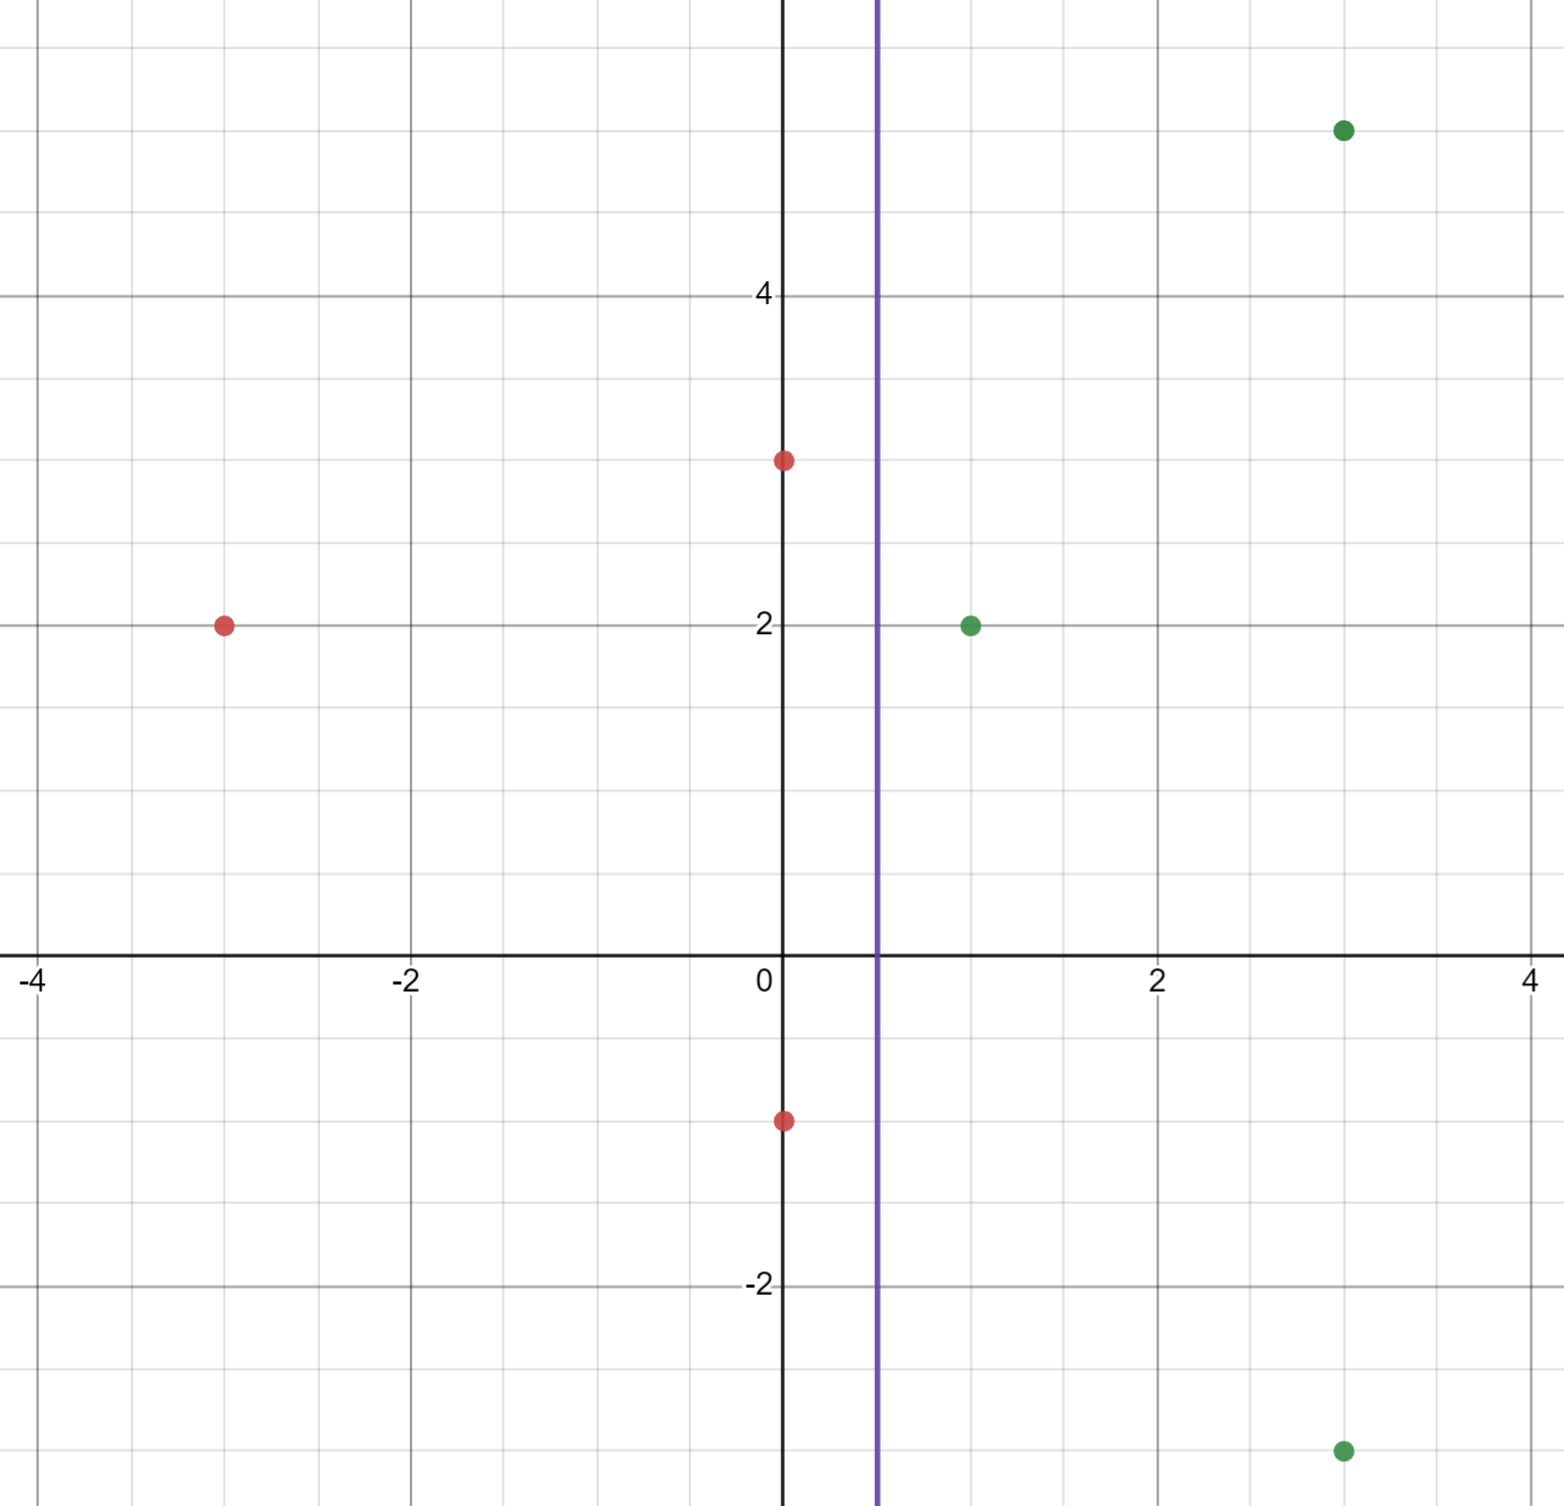
\includegraphics[width=200]{156_final_11.PNG}
\end{center}
When the transformed points are graphed, we see that each classifier lies on a different side of the line $x=0.5$. Thus, only the $z_1$ value for each point matters. To the right of the line, the points are classified as $+1$, and $-1$ on the other side, thus, $w_{z_1}$ is 1, and $w_{z_2}$ is 0. The bias is $-0.5$ as this is the shift of the separating plane. Thus, $w_1=1, w_2=0, b = -0.5$.\\\\ 
\textbf{The answer is [c]}

\section*{problem 12}
See code attached. I get 5 support vectors.\\\\
\textbf{The answer is [c]}

\section*{problem 13}
See code attached. For 100 iterations, the data set generated was never not separable by the RBF kernel. ($0\%$ of the time)\\\\
\textbf{The answer is [a]}

\section*{problem 14}
See code attached. For $K=9$, and $\gamma = 1.5$, the kernel form had a lower $E_{out}$ than the regular form $78\%$ of the time.\\\\
\textbf{The answer is [e]}

\section*{problem 15} 
See code attached. For $K=12$, and $\gamma = 1.5$, the kernel form had a lower $E_{out}$ than the regular form $62.6\%$ of the time.\\\\
\textbf{The answer is [d]}

\section*{problem 16}
See code attached. The frequency of each happening (over 1000 iterations) were as follows:\\
\begin{enumerate}[label = (\alph*)]
    \item 190
    \item 85
    \item 78
    \item 420
    \item 16
\end{enumerate}
\textbf{The answer is [d]}

\section*{problem 17}
See code attached. The frequency of each happening (over 1000 iterations) were as follows:
\begin{enumerate}[label = (\alph*)]
    \item 138
    \item 174
    \item 284
    \item 173
    \item 12
\end{enumerate}
\textbf{The answer is [c]}

\section*{problem 18} 
See attached code. When run over 1000 iterations using $K=0$, and $\gamma=1.5$, the regular RBF achieved $E_{in} = 0$, $1.4\%$ of the time.\\\\
\textbf{The answer is [a]}

\section*{problem 19}
Since $f$ is unknown across the interval $[0, 1]$, and since our random selection had a heart attack, we can describe the posterior probability. Lets say $h$ is closer to 0, $\probP(h=f)$ will be much smaller than when $h$ is near 1. Thus the posterior probability is not uniform. However, as each successive step (regardless of step size) towards 1 from 0 will result in $\probP(h=f)$ to also increase by the same step size. Thus, the posterior probability ($\probP(h=f)$) is linear over $f\in[0, 1]$\\\\
\textbf{The answer is [b]}

\section*{problem 20}
Since we are using mean-squared error, consider some point $\textbf{x}$ that produces $E_{g_1}$ and $E_{g_2}$. Since $g$ is the aggregate of $g_1$ and $g_2$, we know that g(\textbf{x}) will lie somewhere between $g_1(\textbf{x})$ and $g_2(\textbf{x})$. Thus, $E_{g}(\textbf{x})$ will also lie between $E_{g_1}$ and $E_{g_2}$. Thus, $E_{out}(g)$ cannot be worse than the average of $E_{out}(g_1)$ and $E_{out}(g_2)$.\\\\
\textbf{The answer is [c]}


\newpage
{\huge The following code was used to answer questions 7-9:}
\begin{verbatim}
import numpy

def versus_all(n, data_set):
    #splits data and classification info
    data = [[1, data_set[x][1], data_set[x][2], data_set[x][1]*data_set[x][2], data_set[x][1]*data_set[x][1], data_set[x][2]*data_set[x][2]] for x in range(0, len(data_set))]
    classifier = [1 if x[0] == n else -1 for x in data_set]
    return classifier, data

lam = 1

for i in [0, 1, 2, 3, 4, 5, 6, 7, 8, 9]:
    class_i, data_i = versus_all(i, train_data)
    
    X_points = numpy.array(data_i)
    class_array = numpy.array(class_i)
    first_half = numpy.linalg.pinv(numpy.add(numpy.matmul(X_points.T, X_points), lam*numpy.identity(6)))
    w = numpy.matmul(first_half, numpy.matmul(X_points.T, class_array))
    
   
    true_class, test_data_i = versus_all(i, test_data)
    
    test_class_calc = [sign(numpy.dot(test_data_i[x], w)) for x in range(0, len(test_data_i))]
    
    
    E_out = (count_diff(true_class, test_class_calc))/len(true_class)
\end{verbatim}

\newpage
{\huge The following code was used to answer question 10:}
\begin{verbatim}
import numpy

lam = 1

train_1v5 = []
test_1v5 = []

for x in train_data:
    if (x[0] == 1 or x[0] == 5):
        train_1v5.append(x)
        
for x in test_data:
    if (x[0] == 1 or x[0] == 5):
        test_1v5.append(x)
        

                
for lam in [0.01, 1]:
    class_i, data_i = versus_all(1, train_1v5)
    
    X_points = numpy.array(data_i)
    class_array = numpy.array(class_i)
    first_half = numpy.linalg.pinv(numpy.add(numpy.matmul(X_points.T, X_points), lam*numpy.identity(6)))
    w = numpy.matmul(first_half, numpy.matmul(X_points.T, class_array))
    
    true_class, test_data_i = versus_all(1, test_1v5)
    
    test_class_calc = [sign(numpy.dot(test_data_i[x], w)) for x in range(0, len(test_data_i))]
    
    E_out = (count_diff(true_class, test_class_calc))/len(true_class)
    E_in = count_diff([sign(numpy.dot(data_i[x], w)) for x in range(0, len(test_data_i))], class_i)/len(class_i)
    
    print("Lamda: "+str(lam))
    print("E_out: "+str(E_out))
    print("E_in: "+str(E_in))
\end{verbatim}

\newpage
{\huge The following code was used to answer question 12:}
\begin{verbatim}
from sklearn import svm
import numpy
from math import inf

data = [[1, 0], [0, 1], [0, -1], [-1, 0], [0, 2], [0, -2], [-2, 0]]
y = [-1, -1, -1, 1, 1, 1, 1]

clf = svm.SVC(kernel="poly", C=inf, gamma=1, coef0=1)
clf.fit(data, y)  
print(clf.support_vectors_)
\end{verbatim}
\newpage
{\huge The following code was used to answer questions 13-15:}
\begin{verbatim}
import numpy
from random import uniform
from sklearn import svm, cluster
import math

N = 100
gam = 1.5
clusters = 12
iterations = 1000

kernel_wins = 0

for i in range(0, iterations):
    data = [[uniform(-1, 1), uniform(-1, 1)] for x in range(0, N)]
    data_out = [[uniform(-1, 1), uniform(-1, 1)] for x in range(0, N)]
    
    def f(point):
        return sign(point[1] - point[0] + 0.25 * numpy.sin(numpy.pi*point[0]))

    class_data = [f(point) for point in data]
    class_data_out = [f(point) for point in data_out]
    
    clf = svm.SVC(kernel="rbf", C=math.inf, gamma=gam, coef0 = 1)
    clf.fit(data, class_data)  
    
    Kmeans = cluster.KMeans(n_clusters=clusters, init='random').fit(data)
    
    for i in range(0,clusters):
        if (i not in Kmeans.labels_):
            iterations += 1
            continue
    
    phi = numpy.array(build_phi(data, clusters, Kmeans.cluster_centers_))
    class_data = numpy.array(class_data)
    
    w = numpy.matmul(numpy.matmul(numpy.linalg.pinv(numpy.matmul(phi.T, phi)), phi.T), class_data.T)
    
    #KMEANS OUT PREDICTION
    phi_out = numpy.array(build_phi(data_out, clusters, Kmeans.cluster_centers_))
    
    y_out = numpy.matmul(phi_out, w.T)
    y_out = [sign(x) for x in y_out]
    
    E_out_Kmeans = count_diff(y_out, class_data_out)/len(y_out)
    E_out_RBF = count_diff(clf.predict(data_out), class_data_out)/len(data_out)
    
    if E_out_RBF < E_out_Kmeans:
        kernel_wins += 1/iterations
        
def build_phi(points, clusters, centers):
    #BUILD PHI TO GET WEIGHTS
    phi = []
    for m in range(0, len(points)):
        point = points[m]
        row = []
        for n in range(0, clusters):
            center = centers[n]
            temp = numpy.exp(gam*-1 * numpy.linalg.norm(numpy.subtract(point, center))* numpy.linalg.norm(numpy.subtract(point, center)))
            row.append(temp)
        phi.append(row)
    return phi

print(kernel_wins)
\end{verbatim}

\newpage
{\huge The following code was used to answer questions 16-18:}
\begin{verbatim}
import numpy
from random import uniform
from sklearn import svm, cluster
import math

N = 100
gam = 1.5
#clusters = 9
iterations = 1000

answer = [0, 0, 0, 0, 0]

E_i = 0
for i in range(0, iterations):
    compare = []
    for clusters in [9]:
        data = [[uniform(-1, 1), uniform(-1, 1)] for x in range(0, N)]
        data_out = [[uniform(-1, 1), uniform(-1, 1)] for x in range(0, N)]
        
        def f(point):
            return sign(point[1] - point[0] + 0.25 * numpy.sin(numpy.pi*point[0]))

        class_data = [f(point) for point in data]
        class_data_out = [f(point) for point in data_out]

        """clf = svm.SVC(kernel="rbf", C=math.inf, gamma=gam, coef0 = 1)
        clf.fit(data, class_data)  """

        Kmeans = cluster.KMeans(n_clusters=clusters, init='random').fit(data)

        for i in range(0,clusters):
            if (i not in Kmeans.labels_):
                iterations += 1
                continue

        phi = numpy.array(build_phi(data, clusters, Kmeans.cluster_centers_))
        class_data = numpy.array(class_data)

        w = numpy.matmul(numpy.matmul(numpy.linalg.pinv(numpy.matmul(phi.T, phi)), phi.T), class_data.T)

        #KMEANS OUT PREDICTION
        phi_out = numpy.array(build_phi(data_out, clusters, Kmeans.cluster_centers_))

        y_out = numpy.matmul(phi_out, w.T)
        y_out = [sign(x) for x in y_out]
        
        y_in = numpy.matmul(phi, w.T)
        y_in = [sign(x) for x in y_in]

        E_out_Kmeans = count_diff(y_out, class_data_out)/len(y_out)
        E_in_Kmeans = count_diff(y_in, class_data)/len(y_in)
        compare.append(E_out_Kmeans)
        compare.append(E_in_Kmeans)
    
    if compare[1] == 0:
        E_i += 1/iterations
        
    E_in_goes_up = compare[1] < compare[3]
    E_in_goes_down = compare[1] > compare[3]
    E_out_goes_up = compare[0] < compare[2]
    E_out_goes_down = compare[0] > compare[2]
    no_change = bool((compare[1] == compare[3]) & (compare[0] == compare[2]))
    if E_in_goes_down & E_out_goes_up:
        answer[0] += 1
    
    if E_in_goes_up & E_out_goes_down:
        answer[1] += 1
    
    if E_in_goes_up & E_out_goes_up:
        answer[2] += 1
        
    if E_in_goes_down & E_out_goes_down:
        answer[3] += 1
        
    if no_change:
        answer[4] += 1
print(answer)
\end{verbatim}
\end{document}
